\documentclass[12pt]{article}
\usepackage[margin=2.5cm]{geometry}
\usepackage{enumerate}
\usepackage{amsfonts}
\usepackage{amsmath}
\usepackage{fancyhdr}
\usepackage{amsmath}
\usepackage{amssymb}
\usepackage{amsthm}
\usepackage{graphicx}
\usepackage{mdframed}

\begin{document}
\title{Worksheet 4 Review 2}
\maketitle

\section*{Question 1}
\begin{enumerate}[a.]
    \item $\exists n \in \mathbb{N},\:n > 3 \land n^2 -1.5n \geq 5$
    \item The variable is existentially quantified
    \item Because the variable is existentially quantified, the variable's value
    should be a \textit{concrete} natural number
    \item

    \textbf{Statement:} $\exists n \in \mathbb{N},\:n > 3 \land n^2 -1.5n \geq 5$

    \bigskip

    \begin{proof}
    Let $n = 5$.

    \bigskip

    We will prove $n > 3 \land n^2 -1.5n \geq 5$.

    \bigskip

    First, we need to prove $n > 3$.

    \bigskip

    The header tells us $n=5$.

    \bigskip

    Using this fact, we can conclude $n > 3$.

    \bigskip

    Now, we need to show $n^2 - 1.5n \geq 5$.

    \bigskip

    Using the fact $n = 5$, we can calculate

    \begin{align}
        n^2 - 1.5n &= 25 - 7.5\\
        &= 17.5\\
        &\geq 5
    \end{align}

    \bigskip

    Finally, since $n > 3$ and $n^2 - 1.5n \geq 5$ are true, we can conclude
    $n > 3 \land n^2 - 1.5n \geq 5$ are true.
    \end{proof}

    \bigskip

    \textbf{Notes:}

    \begin{itemize}
        \item Used the following pseudoproof used for this problem. Proof really
        feels smoother.

        \begin{center}
        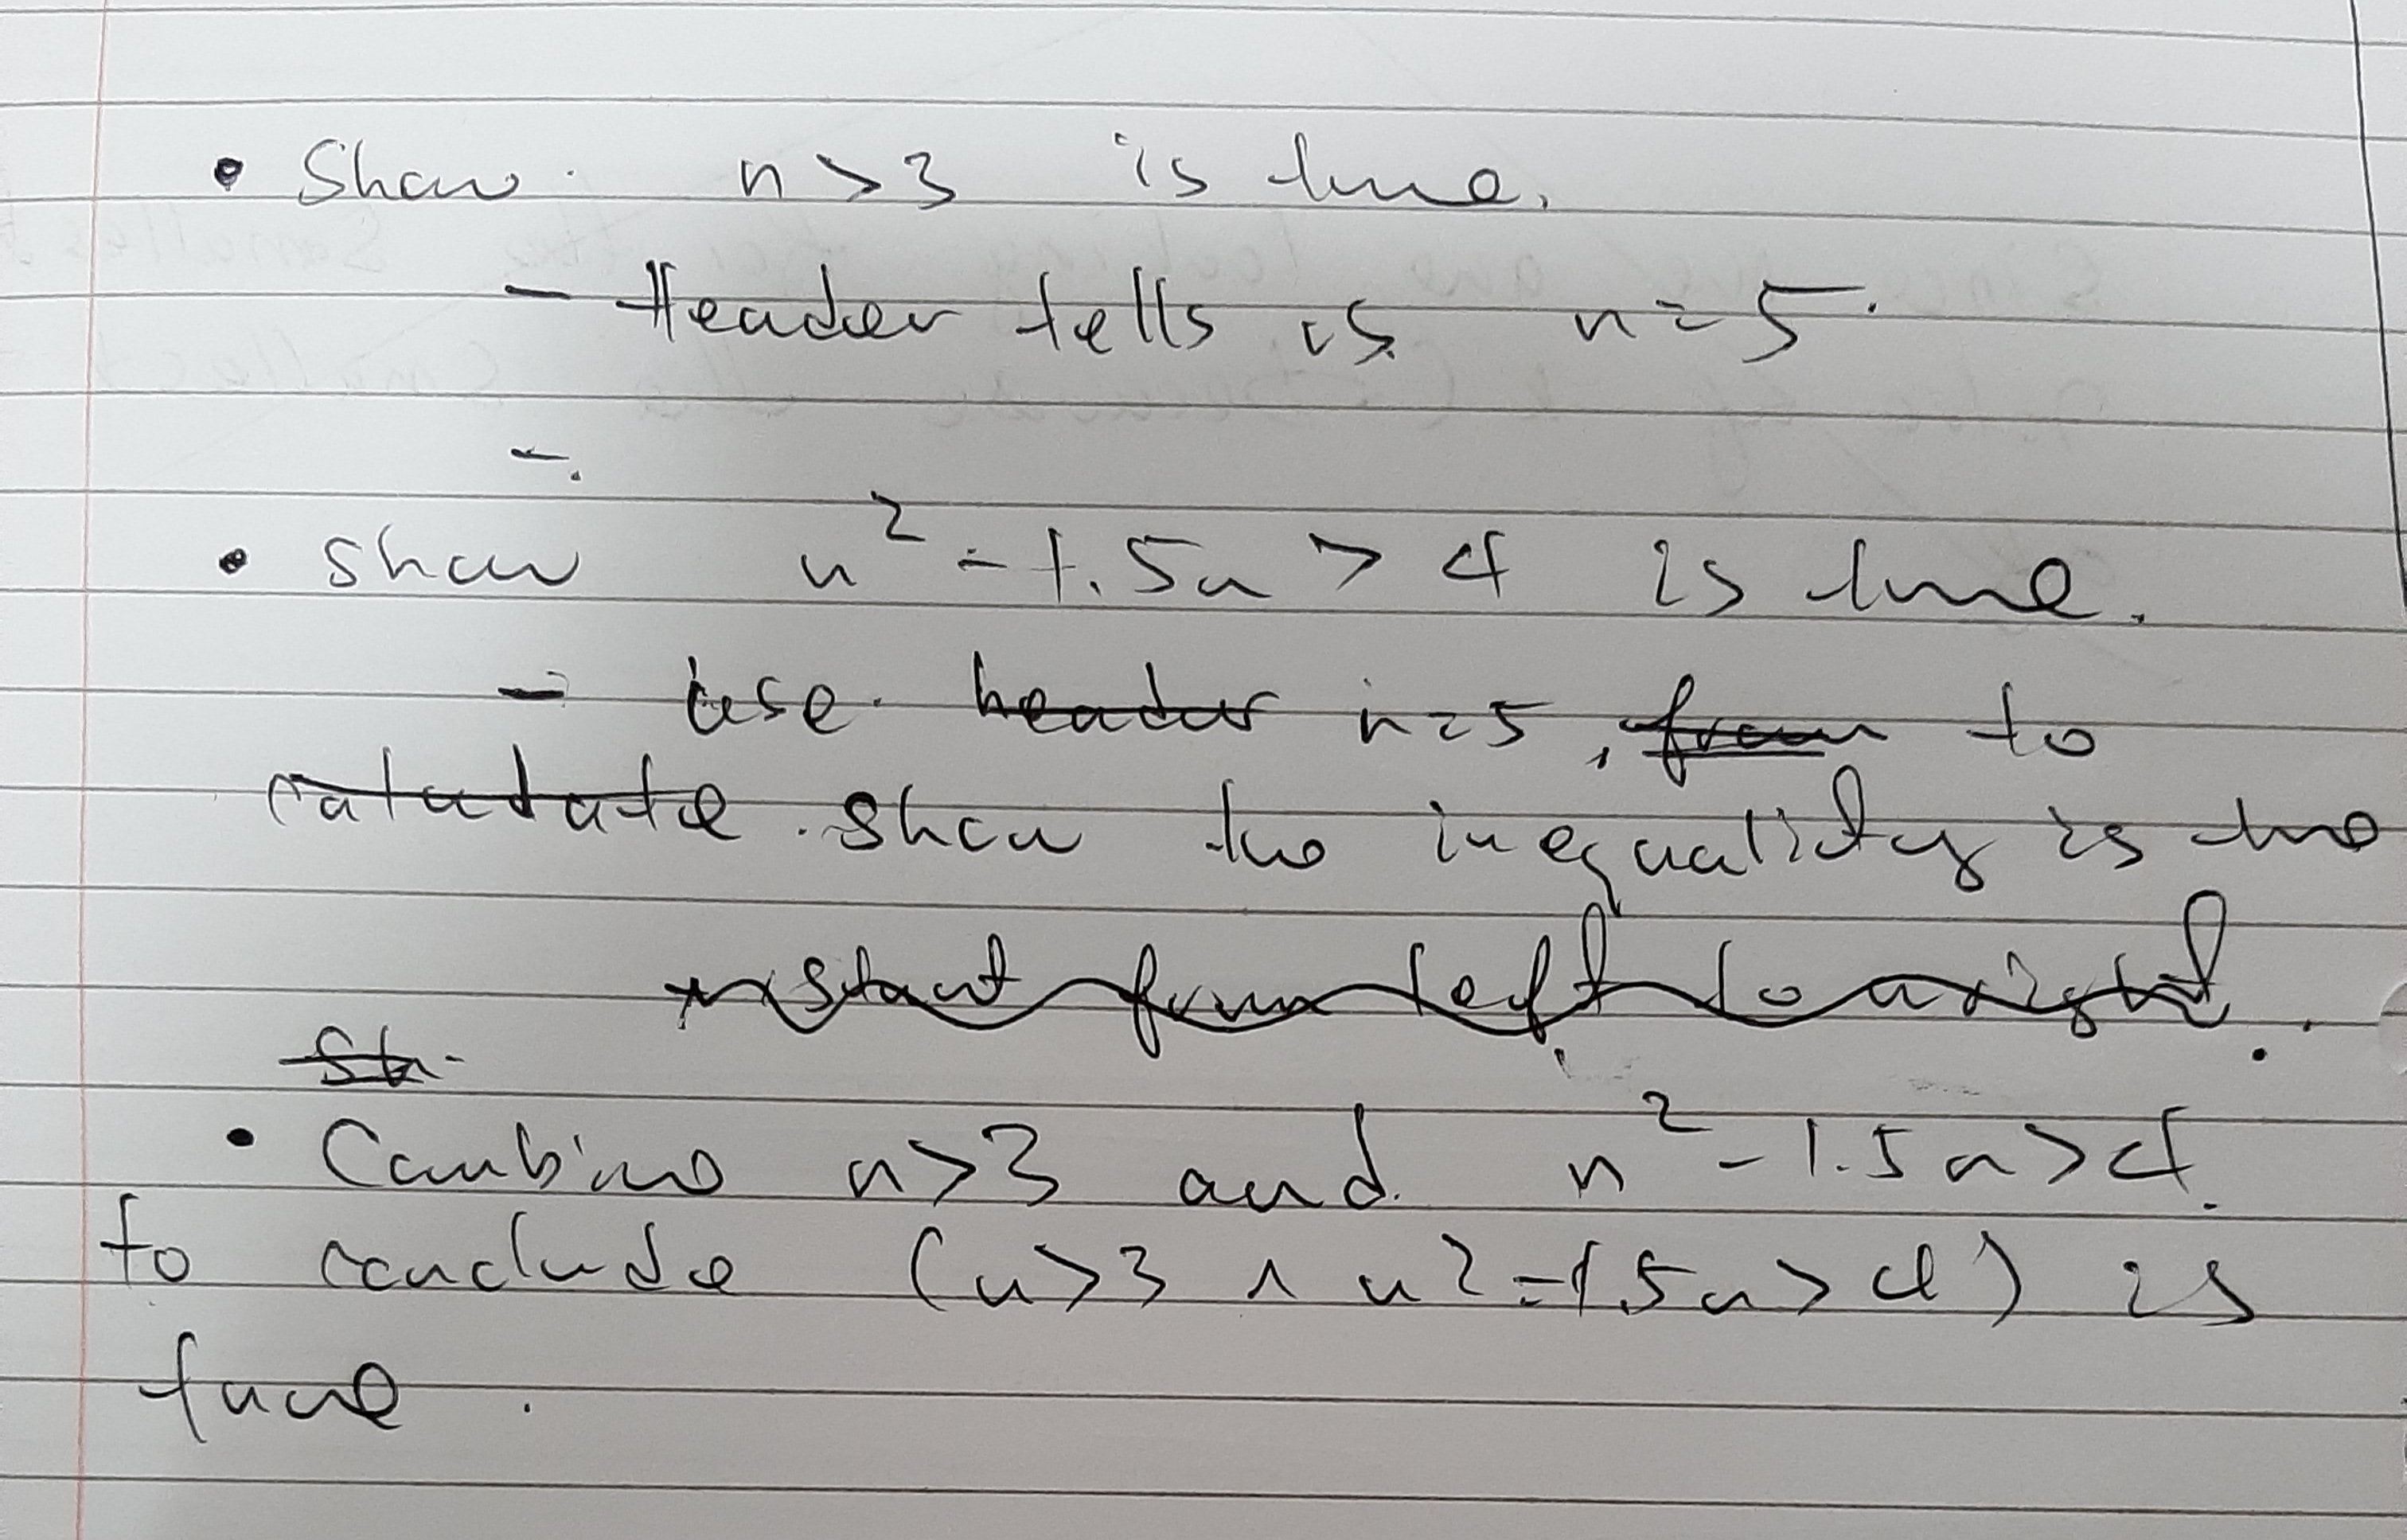
\includegraphics[width=\linewidth]{images/worksheet_4_review_2_q1d_comments.jpg}
        \end{center}

    \end{itemize}

    \item $\forall n \in \mathbb{N},\:n \geq 3 \Rightarrow n^2 - 1.5n > 4$

    \item The variable is universally quantified.

    \item Because the variable is universally quantified, the variable's value
    should be an arbitrary natural number.

    \item

    The assumption made is $n > 3$.

    \bigskip

    This conclusion is made by looking at the L.H.S of the $\Rightarrow$
    operator.

    \item

    \textbf{Statement:} $\forall n \in \mathbb{N},\:n > 3 \Rightarrow n^2 -1.5n > 4$

    \begin{proof}
        Let $n \in \mathbb{N}$. Assume $n \geq 3$.

        \bigskip

        We will prove $n^2 - 1.5n > 4$.

        \bigskip

        Using the fact $n \geq 3$, we can conclude

        \setcounter{equation}{0}
        \begin{align}
            n^2 - 1.5n &\geq (3)^2 - 1.5(3)\\
            &= 9 - 4.5\\
            &= 4.5\\
            &> 4
        \end{align}
    \end{proof}

\end{enumerate}

\section*{Question 2}
\begin{enumerate}[a.]
    \item $\forall n \in \mathbb{N},\:n > 5 \Rightarrow 2 \mid n \lor 3 \mid n$
    \item $\exists n \in \mathbb{N},\: n > 5 \land (2 \nmid n) \land (3 \nmid n)$
    \item

    \textbf{Statement:} $\exists n \in \mathbb{N},\: n > 5 \land (2 \nmid n) \land (3 \nmid n)$

    \begin{proof}
        Let $n = 7$.

        \bigskip

        We will prove $n>5 \land (2 \nmid n) \land (3 \nmid n)$.

        \bigskip

        First, we will to prove $n > 5$.

        \bigskip

        The header tells us $n = 7$.

        \bigskip

        Using this fact, we can conclude $n > 5$.

        \bigskip

        Now, we will prove $2 \nmid n$.

        \bigskip

        7 is a prime number, so we know the number can only be divisible by 1 and 7.

        \bigskip

        Using this fact, we can conclude $2 \nmid 7$.

        \bigskip

        Now, we will prove $3 \nmid n$.

        \bigskip

        Since 7 is divisible by 1 and 7 only, we can conclude $3 \nmid 7$.

        \bigskip

        So, since $n > 5$, $2 \nmid n$ and $3 \nmid n$ are true, we
        can conclude $n>5 \land (2 \nmid n) \land (3 \nmid n)$ holds.
    \end{proof}
\end{enumerate}

\section*{Question 3}

\end{document}